%%%%%%%%%%%%%%%%%%%%%%%%%%%%%%%%%%%%%%%%%%%%%%%%%%%%%%%%%%%%%%%%%%%%
%%%           Vorlage für eine Ausarbeitung an der DHBW          %%%
%%%                                                              %%%
%%%      Bereiche die bearbeitet werden müssen werden durch      %%%
%%%      einen solchen Kommentarblock eingeleitet und enden      %%%
%%%      mit der nächsten Trennlinie.                            %%%
%%%                                                              %%%
%%%      In dieser Datei müssen folgende Bereiche bearbeitet     %%%
%%%      werden:                                                 %%%
%%%      - Angaben zur Arbeit                                    %%%
%%%      - EIGENE KAPITEL EINFÜGEN                               %%%
%%%                                                              %%%
%%%      Benötigte Seiten und Verzeichnisse können unter         %%%
%%%      "Einführung und Verzeichnisse" ein- bzw. auskommentiert %%%
%%%      werden.                                                 %%%
%%%                                                              %%%
%%%%%%%%%%%%%%%%%%%%%%%%%%%%%%%%%%%%%%%%%%%%%%%%%%%%%%%%%%%%%%%%%%%%

\documentclass[a4paper,12pt]{article}
\usepackage[left=2.5cm,right=2.5cm,top=2.5cm,bottom=2.5cm,includehead]{geometry}      % Einstellungen der Seitenränder
\usepackage[english, ngerman]{babel}                                                  % deutsche Silbentrennung
\usepackage[utf8]{inputenc}                                                           % Umlaute
\usepackage[official]{eurosym}                                                        % Euro Symbol
\usepackage[T1]{fontenc}													                                    % Umlaute auch richtig ausgeben
\usepackage{newtxtext,newtxmath}                                                      % Font = Times New Roman
\usepackage{hyperref}
\usepackage[nottoc]{tocbibind}
\usepackage{fancyhdr}
\usepackage{setspace}
\usepackage[backend=bibtex, citestyle=authoryear, bibstyle=authoryear]{biblatex}      % Bibliothek für Zitate
\usepackage{csquotes}                                                                 % Zusatzpacket für Zitate
\usepackage{amsmath}                                                                  % Zurücksetzen der Tabellen- und Abbildungsnummerierung je Sektion
\usepackage[labelfont=bf,aboveskip=1mm]{caption}                                      % Bild- und Tabellenunterschrift (fett)
\usepackage[bottom,multiple,hang,marginal]{footmisc}                                  % Fußnoten [Ausrichtung unten, Trennung durch Seperator bei mehreren Fußnoten]
\usepackage{graphicx}  
\graphicspath{{./images/}}                                                            % Grafiken
\usepackage[dvipsnames]{xcolor}                                                       % Farbige Buchstaben
\usepackage{wrapfig}                                                                  % Bilder in Text integrieren
\usepackage{enumitem}                                                                 % Befehl setlist (Zeilenabstand für itemize Umgebung auf 1 setzen)
\usepackage{listings}                                                                 % Quelltexte
\definecolor{commentgreen}{RGB}{87,166,74}                                            % Kommentar-Farbe für Quellcode
\lstset{numbers=left, numberstyle=\tiny, numbersep=8pt, frame=single, framexleftmargin=15pt, breaklines=true, commentstyle=\color{commentgreen}}
\usepackage{tabularx}                                                                 % Tabellen
\usepackage{multirow}                                                                 % Mehrzeilige Tabelleneinträge
\usepackage[addtotoc]{abstract}                                                       % Abstract
\usepackage[nohyperlinks, printonlyused, withpage]{acronym}                           % Abkürzungen
\usepackage{dirtree}                                                                  % Ordnerstruktur (z.B. für Anhang)

%%%%%%%%%%%%%%%%%%%%%%%%%%%%%%%%%%%%%%%%%%%%%%%%%%%%%%%%%%%%%%%%%%%%
%%%                      Angaben zur Arbeit                      %%%
%%%%%%%%%%%%%%%%%%%%%%%%%%%%%%%%%%%%%%%%%%%%%%%%%%%%%%%%%%%%%%%%%%%%
\def\vFirmenlogoPfad{images/Bosch_DE.png}                  %% relativer Pfad Bsp.: images/Firmenlogo.png
\def\vDHBWLogoPfad{images/DHBW_logo.jpg}                          %% relativer Pfad Bsp.: images/DHBW_logo.jpg
\def\vUnterschrift{}                    %% Pfad zu Bild mit Unterschrift (für digitale Abgabe) Bsp.: images/Unterschrift.png

\def\vTitel{Analyse von Audiosignalen unter der Verwendung von Linear Predictive Coding}                           %% 
\def\vUntertitel{}                      %% 
\def\vArbeitstyp{Projektarbeit}                      %% Projektarbeit/Seminararbeit/Bachelorarbeit
\def\vArbeitsbezeichnung{T3000}              %% T1000/T2000/T3000

\def\vAutor{Henry Schuler}                           %% Vorname Nachname
\def\vMatrikelnummer{5220542}                  %% 7-stellige Zahl
\def\vKursKuerzel{TIT20}                     %% Bsp.: TIT20
\def\vPhasenbezeichnung{Praxisphase}               %% Praxisphase/Theoriephase
\def\vStudienJahr{dritte}                     %% erste/zweite/dritte
\def\vDHBWStandort{Ravensburg}                    %% Bsp.: Ravensburg
\def\vDHBWCampus{Friedrichshafen}                      %% Bsp.: Friedrichshafen
\def\vFakultaet{Technik}                       %% Technik/Wirtschaft
\def\vStudiengang{Informationstechnik}                     %% Informationstechnik/...

\def\vBetrieb{Robert Bosch GmbH}                         %% 
\def\vBearbeitungsort{Blaichach}                 %% 
\def\vAbteilung{TEF-EAT31}                       %% 
\def\vBetreuer{Maximilian Main}                        %% Vorname Nachname

\def\vAbgabedatum{\today}               %% DD. MONTH YYYY
\def\vBearbeitungszeitraum{02.01.2023 - 17.04.2023}            %% DD.MM.YYYY - DD.MM.YYYY


%%%%%%%%%%%%%%%%%%%%%%%%% Eigene Kommandos %%%%%%%%%%%%%%%%%%%%%%%%%
% Definition von \gqq{} und \gq{}: Text in Anführungszeichen
\newcommand{\gqq}[1]{\glqq #1\grqq}
\newcommand{\gq}[1]{\glq #1\grq}
% Spezielle Hervorhebung von Schlüsselwörtern
\newcommand{\textOrdner}[1]{\texttt{#1}}
\newcommand{\textVariable}[1]{\texttt{#1}}
\newcommand{\textKlasse}[1]{\texttt{#1}}
\newcommand{\textFunktion}[1]{\texttt{#1}}


%%%%%%%%%%%%%%%%%%%% Zitatbibliothek einbinden %%%%%%%%%%%%%%%%%%%%%
\addbibresource{./literatur/literatur.bib}


%%%%%%%%%%%%%%%%%%%%%%%% PDF-Einstellungen %%%%%%%%%%%%%%%%%%%%%%%%%
\hypersetup{
  bookmarksopen=false,
	bookmarksnumbered=true,
	bookmarksopenlevel=0,
  pdftitle=\vTitel,
  pdfsubject=\vTitel,
  pdfauthor=\vAutor,
  pdfborder={0 0 0},
	pdfstartview=Fit,
  pdfpagelayout=SinglePage
}


%%%%%%%%%%%%%%%%%%%%%%%% Kopf- und Fußzeile %%%%%%%%%%%%%%%%%%%%%%%%
\pagestyle{fancy}
\setlength{\headheight}{15pt}
\fancyhf{}
\fancyhead[R]{\thepage}


%%%%%%%%%%%%%%%%%%%%%%%%%%%%%% Layout %%%%%%%%%%%%%%%%%%%%%%%%%%%%%%
\onehalfspacing
\setlist{noitemsep}

\addto\captionsngerman{
  \renewcommand{\figurename}{Abb.}
  \renewcommand{\tablename}{Tab.}
}
\numberwithin{table}{section}                               % Tabellennummerierung je Sektion zurücksetzen
\numberwithin{figure}{section}                              % Abbildungsnummerierung je Sektion zurücksetzen
\renewcommand{\thetable}{\arabic{section}.\arabic{table}}   % Tabellennummerierung mit Section
\renewcommand{\thefigure}{\arabic{section}.\arabic{figure}} % Abbildungsnummerierung mit Section
\renewcommand{\thefootnote}{\arabic{footnote}}              % Sektionsbezeichnung von Fußnoten entfernen

\renewcommand{\multfootsep}{, }                             % Mehrere Fußnoten durch ", " trennen


%%%%%%%%%%%%%%%%%%%%%%%%%%%%% Dokument %%%%%%%%%%%%%%%%%%%%%%%%%%%%%

\begin{document}


  %%%%%%%%%%%%%%%%%%% Einführung und Verzeichnisse %%%%%%%%%%%%%%%%%%%
  \pagenumbering{Roman}

  \begin{titlepage}
  \begin{minipage}{6in}
    \vspace*{-2cm}
    \centering
    \hspace{-2cm}
	\ifx\vFirmenlogoPfad\empty
	\else
    \raisebox{-0.5\height}{\includegraphics[height=4cm]{\vFirmenlogoPfad}}
  \fi
	\hfill
	\ifx\vDHBWLogoPfad\empty
	\else
   	\raisebox{-0.5\height}{\includegraphics[height=4cm]{\vDHBWLogoPfad}}
	\fi
  \end{minipage}
  \begin{center}
    \vspace*{0.5cm}
    \Huge\textbf{\vTitel}\\
		\ifx\vUntertitel\empty
		\else
			\Large\rm\vUntertitel\\
		\fi
		\vspace*{2cm}
		\Large\textbf{\vArbeitstyp}
		\ifx\vArbeitsbezeichnung\empty
		\else
			\textbf{\vArbeitsbezeichnung}
		\fi
		\\
		\normalsize
		über die \vPhasenbezeichnung\ des \vStudienJahr{n}\ Studienjahrs \\
		\vspace*{1cm}
		an der Fakultät für \vFakultaet\\
		im Studiengang \vStudiengang\\
		\vspace*{0.5cm}
		an der DHBW \vDHBWStandort\\
		\ifx\vDHBWCampus\empty
		\else
		Campus \vDHBWCampus\\
		\fi
		\vspace*{0.5cm}
		von\\
		\ifx\vAutor\empty
		\else
			\vAutor\\
		\fi
		\vspace*{1cm}
		\vAbgabedatum
		\vfill
  \end{center}
  \begin{tabular}{ll}
    Bearbeitungszeitraum:&\vBearbeitungszeitraum\\
    Matrikelnummer, Kurs:&\vMatrikelnummer, \vKursKuerzel\\
	  Dualer Partner:&\vBetrieb\\
	  Betreuer des Dualen Partners:&\vBetreuer\\
  \end{tabular}
\end{titlepage}
\newpage
\setcounter{page}{2}
  % \thispagestyle{empty}
\section*{\Huge{Sperrvermerk}}

\addcontentsline{toc}{section}{Sperrvermerk}
gemäß Ziffer 1.1.13 der Anlage 1 zu §§ 3, 4 und 5  der Studien- und Prüfungsordnung für die Bachelorstudiengänge im Studienbereich Technik der Dualen Hochschule Baden-Würt­tem­berg vom 29.09.2017.\\

\noindent \gqq{Der Inhalt dieser Arbeit darf weder als Ganzes noch in Auszügen Personen außerhalb des Prüfungsprozesses und des Evaluationsverfahrens zugänglich gemacht werden, sofern keine anders lautende Genehmigung vom Dualen Partner vorliegt.}

\vfill
\leavevmode
\newline
\parbox{6cm}{\strut\centering \vBearbeitungsort, \vAbgabedatum\hrule\strut\centering\footnotesize Ort, Datum} 
\hfill
\ifx\vUnterschrift\empty
\parbox{6cm}{\strut\hspace{1pt} \vAbteilung\hrule\strut\centering\footnotesize Abteilung, Unterschrift}
\else
\parbox{6cm}{\strut\hspace{1pt} \vAbteilung, \parbox[b]{3cm}{\vspace{-10cm}\includegraphics[width=3cm]{\vUnterschrift}}\hrule\strut\centering\footnotesize Abteilung, Unterschrift}
\fi
\vspace{1cm}

\newpage
  \thispagestyle{empty}
\section*{\Huge{Selbstständigkeitserklärung}}

\addcontentsline{toc}{section}{Selbstständigkeitserklärung}
gemäß Ziffer 1.1.13 der Anlage 1 zu §§ 3, 4 und 5  der Studien- und Prüfungsordnung für die Bachelorstudiengänge im Studienbereich Technik der Dualen Hochschule Baden-Würt­tem­berg vom 29.09.2017.

\noindent Ich versichere hiermit, dass ich meine Bachelorarbeit (bzw. Projektarbeit oder Studienarbeit bzw. Hausarbeit) mit dem Thema: 
\begin{center}
	\Large\textbf{\vTitel}
\end{center}
selbstständig verfasst und keine anderen als die angegebenen Quellen und Hilfsmittel benutzt habe. Ich versichere zudem, dass die eingereichte elektronische Fassung mit der gedruckten Fassung übereinstimmt.

\vfill
\leavevmode
\newline
\parbox{6cm}{\strut\centering \vBearbeitungsort, \vAbgabedatum\hrule\strut\centering\footnotesize Ort, Datum} 
\hfill
\ifx\vUnterschrift\empty
\parbox{6cm}{\strut\hspace{1pt} \vAbteilung\hrule\strut\centering\footnotesize Abteilung, Unterschrift}
\else
\parbox{6cm}{\strut\hspace{1pt} \vAbteilung, \parbox[b]{3cm}{\vspace{-10cm}\includegraphics[width=3cm]{\vUnterschrift}}\hrule\strut\centering\footnotesize Abteilung, Unterschrift}
\fi
\vspace{1cm}

\newpage
  \phantomsection
\newenvironment{keywords}{
	\begin{flushleft}
	\small	
	\textbf{
		\iflanguage{ngerman}{Schlüsselwörter}{\iflanguage{english}{Keywords}{}}
	}
}{\end{flushleft}}

% Deutsche Zusammenfassung
\begin{abstract}
	
\end{abstract}

% Schlüsselwörter Deutsch
\begin{keywords}
	
\end{keywords}


\selectlanguage{english}
% Englisches Abstract
\begin{abstract}

\end{abstract}

% Schlüsselwörter Englisch
\begin{keywords}

\end{keywords}


\selectlanguage{ngerman}
\newpage
  \tableofcontents
\newpage
  \section*{Abkürzungsverzeichnis}
\addcontentsline{toc}{section}{Abkürzungsverzeichnis}
\begin{acronym}
  \acro{DHBW}[DHBW]{Duale Hochschule Ba\-den-\-Würt\-tem\-berg}
  \acroplural{DHBW}[DHBW]{Dualen Hochschule Ba\-den-\-Würt\-tem\-berg}
  \acro{FFT}[FFT]{Fast Fourier Transform}
  \acro{LPC}[LPC]{Linear Predicitve Coding}
  \acro{LPCC}[LPCC]{Linear Prediction Cepstral Coefficient}
  \acro{MFCC}[MFCC]{Mel-frequency Cepstral Coefficients}
  \acro{AR}[AR]{Autoregression}
  \acro{NN}[NN]{Neuronales Netz}
  \acroplural{NN}[NN]{Neuronalen Netzes}
\end{acronym}
\newpage
  \listoffigures
\newpage
  \listoftables
\newpage
  \lstlistoflistings
\addcontentsline{toc}{section}{Listings}
\newpage
  % \section*{Vorwort}
\addcontentsline{toc}{section}{Vorwort}
\newpage


  %%%%%%%%%%%%%%%%%%%%%%%%%%%%% Kapitel %%%%%%%%%%%%%%%%%%%%%%%%%%%%%%
  \pagestyle{fancy}
  \fancyhead[L]{\nouppercase{\rightmark}}    % Abschnittsname im Header
  \pagenumbering{arabic}

  %%%%%%%%%%%%%%%%%%%%%%%%%%%%%%%%%%%%%%%%%%%%%%%%%%%%%%%%%%%%%%%%%%%%
  %%%%                   EIGENE KAPITEL EINFÜGEN                  %%%%
  %%%%%%%%%%%%%%%%%%%%%%%%%%%%%%%%%%%%%%%%%%%%%%%%%%%%%%%%%%%%%%%%%%%%
  \section{Einleitung}\label{sec:Einleitung}
Im Rahmen des Informatikstudiums an der \acp{DHBW} Ravensburg muss im dritten Studienjahr eine Studienarbeit abgelegt werden.
Die Hochschule stellt dafür eine Auswahl an Themen zur Verfügung.
Eines dieser Themen beschäftigt sich mit der Problematik der Sprecherauthentifizierung, wobei es Nutzern ermöglicht werden soll, sich über ihre Stimme zu authentifizieren.
In dieser Arbeit sollen die Grundlagen für die Bearbeitung dieser Studienarbeit behandelt werden.

\subsection{Kontext}
Damit ein Zusammenhang zwischen Stimme und Audioaufzeichnung hergestellt werden kann, müssen stimm\-spezifische Merkmale aus dem aufgezeichneten Stimmsignal extrahiert werden.
Im Bereich der Sprecherauthentifizierung haben sich zwei Verfahren zur Berechnung stimm\-spezifischer Merkmale etabliert: \ac{MFCC} und \ac{LPC} \autocite[vgl.][S. 116]{sidorov_text-independent_2010}\autocite[vgl.][S. 726]{chelali_text_2017}.
Während mittels des \ac{MFCC} Verfahrens versucht wird, die Funktionsweise des menschlichen Ohrs abzubilden, versucht das \ac{LPC} Verfahren die Eigenschaften des menschlichen Vokaltrakts aus dem Audiosignal zu extrahieren \autocite[vgl.][S. 117]{sidorov_text-independent_2010}.
Die erhaltenen Werte können anschließend für das Training eines \acp{NN} verwendet werden, welches die Klassifizierung neuer Datensätze während des Authentifizierungsprozesses übernimmt.

\subsection{Ziel der Arbeit}
Im Rahmen dieser Arbeit soll das \ac{LPC} Verfahren genauer untersucht werden.
Dazu soll ein Programm erstellt werden, welches ein gegebenes Audiosignal mittels \ac{LPC} in eine vordefinierte Anzahl an Koeffizienten umwandelt.
In einem weiteren Schritt soll der Zusammenhang zwischen den berechneten Koeffizienten und der sprechenden Person unter Verwendung eines vereinfachten \acp{NN} aufgezeigt werden.

\subsection{Vorgehensweise}
% 2. Grundlagen: Signalvorverarbeitung + LPC berechnung
% 3. Technische Umsetzung: Applikation
% 4. Validierung: NN Aufbau + Ergebnis.
% 5. Kritische Reflexion und Ausblick
Die Arbeit unterteilt sich in fünf Kapitel.
Im Anschluss an die Einleitung stellt Kapitel~\ref{sec:Grundlagen} die für diese Arbeit relevanten Grundlagen vor.
Kapitel~\ref{sec:TechnischeUmsetzung} kombiniert die vorgestellten Verfahren zu einem ausführbaren Programm.
Die Ergebnisse des erstellten Programms werden in Kapitel~\ref{sec:Validierung} validiert.
Abschließend werden die Erkenntnisse in Kapitel~\ref{sec:Ausblick} interpretiert und die Arbeit wird mit einem Ausblick abgeschlossen.
  \section{Grundlagen}\label{sec:Grundlagen}
\subsection{Signalvorverarbeitung}
Um ein gegebenes Audiosignal einheitlich verarbeiten zu können, muss dieses zunächst mittels verschiedener Verfahren vorbereitet werden.
Ziel dieser Vorverarbeitung ist es, die Effizienz und Effektivität des anschließenden Verarbeitungsprozess zu erhöhen und somit ein verbessertes Ergebnis zu erzielen \autocite[vgl.][S. 11672]{lokesh_speech_2019}.
Die Vorverarbeitung im Rahmen dieser Arbeit beschränkt sich auf die beiden Schritte Framing und Windowing, welche in den folgenden Unterkapiteln genauer erläutert werden.

\subsubsection{Framing}
Das Unterteilen von Audiosignalen in kleinere Blöcke (Frames) wird als Framing bezeichnet.
Dabei muss zunächst eine einheitliche Blockgröße festgelegt werden.
Außerdem wird eine Überlagerungszeit definiert, welche eine Überlappung der einzelnen Blöcke verursacht.
% TODO: Quelle hinzufügen
% TODO: Warum wird überlagert -> Quelle

\subsubsection{Windowing (Zeitfenster)}
\begin{figure}
  \centering
  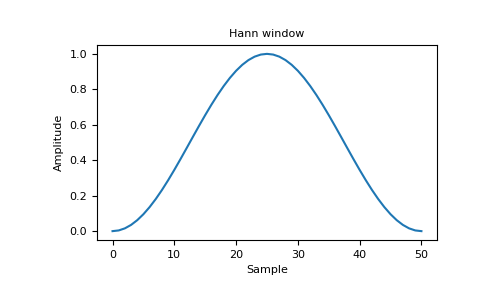
\includegraphics[width=0.8\textwidth, keepaspectratio]{images/hann_window.png}
  \caption{Von Hann Fensterfunktion \autocite{noauthor_numpyhanning_nodate}}
  \label{fig:vonHannFenster}
\end{figure}
Um die bei der Unterteilung des Audiosignals entstandenen Diskontinuitäten aufzulösen, wird eine Fensterfunktion auf die einzelnen Blöcke angewendet.
Abbildung~\ref{fig:vonHannFenster} zeigt die von Hann Fensterfunktion, welche neben dem Hamming Fenster zu den typischen Fensterfunktionen in der Audiosignalverarbeitung zählt.
Durch den Nulldurchgang am Anfang und Ende der Fensterfunktion werden die Amplituden des Blocksignals nach Anwenden der Funktion an den Grenzen auf Null gezogen, wodurch sich ein kontinuierlicher, periodischer Signalverlauf ergibt.
Dieser wird von den in dieser Arbeit verwendeten Funktionen wie etwa der \ac{FFT} vorausgesetzt.

Wird der Schritt des Windowing nicht durchgeführt, führt dies zu einem Phänomen namens Spectral leakage.
Der Amplitudensprung an den Blockenden resultiert in der Registrierung einer vielzahl von Frequenzen, welches die korrekte Ermittlung der sich im Signal befindenden Frequenzen erschwert.
Wie der Name bereits beschreibt, wird aus einer eindeutigen Frequenz, ein Spektrum aus Frequenzen.
% TODO: Wird Windowing in diesem Anwendungsfall überhaupt benötigt?

\begin{itemize}
  \item Spektral leakage
  \item Hamming und Han Fenster
  \item Unterschied zu Framing
\end{itemize}
\subsection{Auto regressive moving average filter}
% TODO: Was ist es + was hat es mit LPC zu tun

\subsection{Cepstral vectors/coefficients}
% TODO: Was sind Cepstral coefficients
% TODO: Warum werden sie verwendet, was ist der Vorteil?

  \section{Technische Umsetzung}\label{sec:TechnischeUmsetzung}
  \section{Validierung}\label{sec:Validierung}
Damit sichergestellt werden kann, dass die in dieser Arbeit erarbeitete Parametrisierung von Stimmaufzeichnungen eine Aussage über die jeweilige sprechende Person ermöglicht, muss der Zusammenhang zwischen den berechneten \ac{LPC} Koeffizienten und der sprechenden Person gezeigt werden.
Dies erfolgt in der Klasse \textKlasse{FeatureEvaluator} (vgl. Quellcode~\ref{code:FeatureEvaluator}).

Hierfür wird wie bereits eingangs erwähnt ein einfaches \ac{NN} mit Hilfe der Python-Bibliothek \textKlasse{tensorflow} trainiert.
Das \ac{NN} besteht dabei aus einem Input-Layer mit 30 * 12 Features = 360 Neuronen, zwei Hidden-Layern mit je 16 Neuronen, sowie einem Output-Layer (vgl. Z.~\ref{line:NNStart}-\ref{line:NNEnd}).
Da im Output-Layer für jede Sprecher-ID ein Neuron erstellt wird, passt sich die Anzahl der Neuronen an die höchste verwendete Sprecher-ID an (vgl. Z.~\ref{line:NNOutput}).
\newline
\newline
Als Datengrundlage kommt ein von Vibhor Jain erstellter Datensatz zum Einsatz, welcher auf der Internetseite kaggle.com zur Verfügung steht und Audio-Datensätze zu 50 unterschiedlichen Sprechern bereitstellt \autocite[vgl.][]{vibhor_jain_speaker_2019}.
Für jeden Sprecher existieren dabei Aufzeichnungen mit einer Dauer von bis zu einer Stunde, welche in einminütige WAV-Dateien heruntergebrochen wurden.
Die Dateien mit Index null bis einschließlich 14 jedes Sprechers werden zum Training des \ac{NN} verwendet.
Alle Dateien ab Index 15 können somit zum Testen des \ac{NN} verwendet werden.

Für die Generierung der Trainingsdaten für das \ac{NN} wird der in Kapitel~\ref{sec:TechnischeUmsetzung} beschriebene Ablauf durchgeführt.
Dabei wird eine Blockgröße von 500 Samples mit einer Überlappung von 100 Samples gewählt.
Für die Personen 21 bis 30 werden je 1000 Chunks bestehend aus jeweils 30 aufeinanderfolgenden Frames generiert.
Da für jeden Frame zwölf Koeffizienten berechnet werden, enthält jeder Chunk somit 360 \ac{LPC} Werte.
Für eine einfach skalierbare Erstellung des Datensatzes wird die Funktion \textFunktion{create\_dataset} (vgl. Z.~\ref{line:createDatasetStart}-\ref{line:createDatasetEnd}) verwendet, welche neben dem erstellten Datensatz eine weitere Liste, die die Zuordnung des Datensatzes zu der Sprecher-ID enthält, zurückgibt.

Bevor die Trainingsdaten nun für das Training des \ac{NN} verwendet werden, werden diese gemischt, um ein besseres Trainings-Ergebnis zu erzielen (vgl. Z.~\ref{line:shuffle}).
\newline
\newline
Für die Evaluation des trainierten Modells, wird ein Test-Datensatz nach dem selben Verfahren aus den Dateien ab Index 15 für die Personen 21 bis 30 erstellt.
Somit wird zunächst sichergestellt, dass es sich bei den Testdaten um unbekannte Werte für das \ac{NN} handelt.

Mit der Funktion \textFunktion{evaluate\_model} (vgl. Z.~\ref{line:evaluateModelStart}-\ref{line:evaluateModelEnd}) kann nun die Genauigkeit, sowie die Fehlerrate des \ac{NN} ermittelt werden.
Der in dieser Arbeit verwendete Test-Datensatz wurde von dem Modell zu 70,54 Prozent korrekt vorhergesagt, bei einer Fehlerrate von 5,47.
Die Fehlerrate berechnet sich dabei nach dem categorical crossentropy Verfahren.

\begin{table}
  \centering
  \begin{tabular}{|cc*{10}{|r}|}
    \hline
    \multicolumn{2}{|c|}{}&\multicolumn{10}{c|}{\textsf{Testdaten Sprecher ID}}\\
    &             &     \textbf{21} &     \textbf{22} &     \textbf{23} &     \textbf{24} &     \textbf{25} &     \textbf{26} &     \textbf{27} &     \textbf{28} &     \textbf{29} &     \textbf{30} \\
    \hline
    & \textbf{21} &    \textbf{437} &               3 & \underline{233} & \underline{229} &              31 &               0 &               0 &               0 &               1 &               0 \\
    & \textbf{22} &               2 &    \textbf{560} &               0 &               0 &               0 &              11 &              22 &              74 &              22 &              39 \\
    & \textbf{23} & \underline{258} &               0 &    \textbf{701} &              15 &              24 &               0 &               0 &               0 &               0 &               0 \\
    & \textbf{24} &             257 &               0 &              33 &    \textbf{743} & \underline{ 33} &               0 &               0 &               0 &               0 &               0 \\
    & \textbf{25} &              46 &              12 &              33 &              13 &    \textbf{912} &               0 &               0 &               0 &               0 &               0 \\
    & \textbf{26} &               0 &              47 &               0 &               0 &               0 &    \textbf{535} & \underline{193} &              25 &              37 &              40 \\
    & \textbf{27} &               0 &              64 &               0 &               0 &               0 &             142 &    \textbf{771} &               1 &              10 &               3 \\
    & \textbf{28} &               0 & \underline{146} &               0 &               0 &               0 &             136 &               5 &    \textbf{779} &              59 & \underline{ 83} \\
    & \textbf{29} &               0 &              67 &               0 &               0 &               0 & \underline{154} &               6 &              37 &    \textbf{796} &              15 \\
    \smash{%
      \lower\dimexpr\dp\csname @arstrutbox\endcsname-\dp\strutbox+\arrayrulewidth\relax
      \hbox{\rotatebox[origin=bl]{90}{%
        \textsf{%
          %\fboxsep=-\fboxrule
          %\fbox{%
          \parbox[b]{\dimexpr 10\dp\csname @arstrutbox\endcsname+10\ht\csname @arstrutbox\endcsname\relax}{%
            \centering
            \strut Zugeordnete Sprecher ID\strut
            }%
            %}%
            }%
            }}%
            }%
            & \textbf{30} &               0 &             101 &               0 &               0 &               0 &              22 &               5 & \underline{ 84} & \underline{ 75} &    \textbf{820} \\
            \hline
            \hline
    \multicolumn{2}{|c|}{\textbf{Abstand zu 2}} & 179 & 414 &         468 &             514 &             879 &             381 &             578 &             695 &             721 &             737\\
    \hline
  \end{tabular}
  \caption{Modell Vorhersagen für 1000 Testdaten pro Sprecher}
  \label{tab:ModellPredictions}
\end{table}

Betrachtet man die Vorhersagen des Modells mittels der Funktion \textFunktion{predict} (vgl. Z.~\ref{line:predictStart}-\ref{line:predictEnd}) genauer, ergibt sich die in Tabelle~\ref{tab:ModellPredictions} dargestellte Verteilung.
Es ist zu erkennen, dass das Modell jeden Sprecher korrekt vorhergesagt hat, wobei die Zuversichtlichkeit im schlechtesten Fall 43,7 und im besten Fall 91,2 Prozent beträgt.
Zwischen dem Vorhergesagten Sprecher (fett) sowie dem Sprecher mit den zweitmeisten Vorhersagen (unterstrichen) liegt dabei im Durchschnitt ein Abstand von 55,7 Prozentpunkten.
Relativ betrachtet wird der korrekte Sprecher im Durchschnitt 4,7 Mal so oft wie der Sprecher mit den zweitmeisten Vorhersagen zugeordnet.
  \section{Kritische Reflexion und Ausblick}\label{sec:Ausblick}
In dieser Arbeit wurde ein lineares Verfahren entwickelt, welches Audiodateien zunächst in vier sequenziellen Schritten vorverarbeitet und anschließend in \ac{LPC} Koeffizienten umrechnet.
Der theoretische Ansatz hinter der \ac{LPC} Berechnung zeigt dabei bereits ein hohes Potenzial der Koeffizienten für die Verwendung im Kontext Sprecherauthentifizierung.

Im Rahmen der Implementierung der vorgestellten Verfahren wird auf einen modularen Ansatz gesetzt, der eine Erweiterung des entwickelten Programms um verschiedene Verfahren der Koeffizientenberechnung ermöglicht, wodurch dieses als Basis für die anschließende Studienarbeit verwendet werden kann.
Gleichzeitig können relevante Größen wie die Länge der zu erstellenden Frames oder die Anzahl zu berechnender Koeffizienten als Parameter den entsprechenden Funktionen übergeben werden, wodurch eine hohe Flexibilität erreicht wird.

Die abschließende Validierung der Ergebnisse dieser Arbeit bestätigen die in der Einleitung getroffene These.
Mit einer Genauigkeit von 70,54 Prozent kann das trainierte \ac{NN} neue Stimmaufzeichnungen den korrekten Sprechern zuordnen.
Es besteht somit ein klarer Zusammenhang zwischen den berechneten Koeffizienten und der sprechenden Person.
Dabei kann mit Blick auf die begrenzten Testdaten festgestellt werden, dass der korrekte Sprecher im Durchschnitt 4,7 Mal so oft gegenüber dem Sprecher mit den zweitmeisten Vorhersagen zugeordnet wird, was die Effektivität der Koeffizienten noch einmal verstärkt hervorhebt.
\newline
\newline
Im Kontext der anschließenden Studienarbeit zeigen die Ergebnisse, dass die \ac{LPC} Koeffizienten gewinnbringend für die Authentifizierung von Sprechern sind.
Diese Arbeit bietet somit die Grundlage für verschiedene Ansätze, die im Rahmen der Studienarbeit aufgefasst und vertieft werden können.

Durch Anpassungen der Koeffizienten-Zusammensetzung kann untersucht werden, ob die Genauigkeit des \ac{NN} verbessert werden kann.
Dies bezieht sich insbesondere auf die Faktoren Vorhersagegenauigkeit und Fehlerrate des \ac{NN}.

Neben der Koeffizienten-Zusammensetzung kann der Fokus ebenfalls auf den Aufbau des \ac{NN} gelegt werden.
Das in dieser Arbeit verwendete Netz beschreibt einen standard-Aufbau eines \ac{NN} und ist somit nicht für die Sprecherauthentifizierung optimiert.
Es kann untersucht werden, inwiefern eine Veränderung der Schichtgrößen, sowie der allgemeinen Struktur zu einer Verbesserung der Vorhersagegenauigkeit und Fehlerrate führt.

Als dritte Option besteht die Möglichkeit der Erweiterung des entwickelten \ac{LPC} Verfahrens.
Durch weitere Rechenschritte können \ac{LPC} Koeffizienten in \ac{LPCC} umgerechnet werden.
Im Rahmen einer Anschlussarbeit kann evaluiert werden, ob die Umrechnung in \ac{LPCC} zu einer Verbesserung der Sprecherauthentifizierung führt.

  %%%%%%%%%%%%%%%%%%%%%%% Literaturverzeichnis %%%%%%%%%%%%%%%%%%%%%%%
  \phantomsection
\addcontentsline{toc}{section}{Literatur}
\printbibliography
\newpage


  %%%%%%%%%%%%%%%%%%%%%%%%%%%%%% Anhang %%%%%%%%%%%%%%%%%%%%%%%%%%%%%%
  \renewcommand{\thetable}{\Alph{section}.\arabic{table}}
  \renewcommand{\thefigure}{\Alph{section}.\arabic{figure}}
  \renewcommand{\thelstlisting}{\Alph{section}.\arabic{lstlisting}}
  \pagenumbering{Alph}

  \begin{appendix}
  \section{Anhang}
  \subsection{AudioPreprocessor}
  \lstset{escapeinside={\#(*@}{@*)}}
  \lstinputlisting[caption={Signalvorverarbeitung}, captionpos=b, language=Python, label=code:AudioPreprocessor]{code/preprocessing/AudioPreprocessor.py}
\end{appendix}
\end{document}